\documentclass{report}

\usepackage{amsmath}
\usepackage[inline]{enumitem}  % enumerate
\usepackage{listings}
\usepackage{tikz}
%\usepackage{forest}

\usetikzlibrary{patterns}
\usetikzlibrary{positioning}

\lstset{
	basicstyle=\ttfamily,
	columns=fullflexible,  % thanks https://tex.stackexchange.com/a/172705
	keepspaces=true,
}

%\forestset{
%	default preamble={
%		for tree={circle,draw},
%		/tikz/every node/.append style={font=\footnotesize},
%	}
%}

\begin{document}

\chapter{Introduction to algorithm design}

n/a

\chapter{Algorithm analysis}

\section*{Notes}
The dominance pecking order:
\begin{gather*}
	n! \gg c^n \gg n^3 \gg n^2 \gg n^{1+\epsilon} \gg n\log n \gg n \gg \sqrt{n} \gg \\
	\log^2 n \gg \log n \gg \log n/\log\log n \gg \log\log n \gg \alpha(n) \gg 1
\end{gather*}

\section*{Solutions}
\paragraph{2-10}
\begin{enumerate}[label=(\alph*)]
	\item $f(n) = (n^2 - n)/2,\ g(n) = 6n.$

		Is $f(n) = O(g(n))$? If so, there is $c$ such that $f(n) \le cg(n)$
		for sufficiently large $n$.
		\begin{equation*}
			\frac{1}{2}\left(n^2 - n\right) \le 6n
				\ \rightarrow\ n^2 - n \le 12n
				\ \rightarrow\ n(n-1) \le 12n
		\end{equation*}
		Suppose there is such a $c$, then
		\begin{equation*}
			n(n-1) \le 12cn\ \rightarrow\ n-1 \le 12c
		\end{equation*}
		Clearly we can always find $n$ such that this inequality won't hold,
		so $f(n) \ne O(g(n))$.

		Is $g(n) = O(f(n))$? If so, there is $c$ such that $g(n) \le cf(n)$
		for sufficiently large $n$.
		\begin{equation*}
			6n \le \frac{1}{2}\left(n^2 - n\right)
			\ \rightarrow\ 12n \le n^2 - n = n(n-1)
			\ \rightarrow\ 12 \le n - 1
			\ \rightarrow\ 13 \le n.
		\end{equation*}
		So with $c = 1$ the inequality will hold for $n_0 \ge 13$, and $g(n) = O(f(n))$.

	\item $f(n) = n + 2\sqrt{n},\ g(n) = n^2.$

		$f(n) = O(g(n)) \Leftrightarrow f(n) \le cg(n)$ for sufficiently large $n$.
		\begin{gather*}
			n + 2\sqrt{n} \le cn^2,\ \text{with}\ c = 1, \\
			n + 2\sqrt{n} \le 2n\ \text{for $n > 4$}, \\
			2n \le n^2\ \text{so}\ f(n) = O(g(n)).
		\end{gather*}

		$g(n) = O(f(n)) \Leftrightarrow g(n) \le cf(n)$ for sufficiently large $n$. But
		this asks to find $c$ such that $n^2 \le c\left(n + 2\sqrt{n}\right)$; since
		ultimately $n^2 \gg n$, $g(n) \ne O(f(n))$.

	\item $f(n) = n\log n,\ g(n) = n\sqrt{n}.$
		\begin{gather*}
			f(n) = O(g(n)) \Leftrightarrow n\log n \le cn\sqrt{n},\ \text{with $c=1,$} \\ 
			\rightarrow\ \log n \le \sqrt{n/2},
		\end{gather*}
		since $\sqrt{n} \gg \log n,\ f(n) = O(g(n)).$

		By the same argument, $g(n) \ne O(f(n)).$

	\item $f(n) = n + \log n,\ g(n) = \sqrt{n}\ \rightarrow\ n + \log n \le c\sqrt{n}$, and
		since $n \gg \sqrt{n}$, any constant factor will be dominated by the linear term, so
		$f(n) \ne O(g(n)).$ Conversely and by the same argument, $g(n) = O(f(n)).$

	\item $f(n) = 2\left(\log n\right)^2,\ g(n) = \log n + 1.$ Note that
		$2\left(\log n\right)^2 = 2\log^2 n$, and $\log^2 n \gg \log n,$ so $g(n) = O(f(n))$
		and $f(n) \ne O(g(n)).$

	\item $f(n) = 4n\log n + n,\ g(n) = \left(n^2 - n\right)/2.$ We know that
		$n\log n \gg n,$ so we can consider just this term from $f(n).$ But ultimately the
		quadratic term in $g(n)$ dominates so $f(n) = O(g(n)).$
\end{enumerate}


\paragraph{2-11}
\begin{enumerate}[label=(\alph*)]
	\item $f(n) = 3n^2,\ g(n) = n^2.$

		With $c = 3,\ f(n) \le 3g(n)$ so $f(n) = O(g(n)).$

		$f(n) = \Omega(n) \Leftrightarrow cg(n) \le f(n)$ for sufficiently large $n$. For
		$c = 1$ the inequality holds, so $f(n) = \Omega(g(n))$ and $f(n) = \Theta(g(n)).$

	\item $f(n) = 2n^4 - 3n^2 + 7,\ g(n) = n^5.$
	
		$n^5 \gg n^4$ so $f(n) = O(g(n))$ and $f(n) \ne \Omega(g(n)).$

	\item $f(n) = \log n,\ g(n) = \log n + \frac{1}{n}.$

		$\lim_{n\rightarrow\infty} \frac{1}{n} = 0,$ so as $n\rightarrow\infty$,
		$f(n) - g(n) = 0$. So no function dominates the other. Thus, $f(n) = \Theta(g(n)).$

	\item $f(n) = 2^{k\log n},\ g(n) = n^k.$
		\begin{gather*}
			f(n) = O(g(n)) \Leftrightarrow f(n) \le cg(n) \\
			\rightarrow\ 2^{k\log n} \le cn^k;\ \text{taking logarithms,} \\
			\rightarrow\ \log\left(2^{k\log n}\right) \le \log\left(cn^k\right)
				= \log c + \log n^k \\
			\rightarrow\ k\log n\log 2 \le \log c + k\log n.
		\end{gather*}
		Ignoring constant terms and multiplicative constants, we are left with
		$\log n \le \log n$, so $f(n) = \Theta(g(n)).$

	\item $f(n) = 2^n,\ g(n) = 2^{2n}.$

		$2^n \le c2^{2n}$ clearly holds for $c = 1$, so $f(n) = O(g(n)).$

		$c2^{2n} \le 2^n$? Well, $2^{2n} = 2^2\cdot2^n = 4\cdot2^n,$ so
		$4c2^n \le 2^n$ is satisfied with $c = 1/4.$ So $f(n) = \Omega(g(n))$ and
		finally, $f(n) = \Theta(g(n)).$
\end{enumerate}

\paragraph{2-12}$n^3 - 3n^2 -n + 1 = \Theta\!\left(n^3\right).$

Note that $0 \le 3n^2 + n \rightarrow n^3 \le n^3 + 3n^2 + n \rightarrow n^3 - 3n^2 - n \le n^3$. Thus $f(n) = O\left(n^3\right)$.

Now $cn^3 \le n^3 - 3n^2 - n + 1.$ Consider $c = 1/2$, then
\begin{align*}
	n^3/2 &\le n^3 - 3n^2 - n + 1 \\
	-n^3/2 &\le -3n^2 - n + 1 \\
	-n^3 &\le -6n^2 - 2n + 2 \\
	n^3 &\ge 6n^2 + 2n - 2. 
\end{align*}
This holds for $n_0 \ge 7$, so $f(n) = \Omega\!\left(n^3\right)$ and finally $f(n) = \Theta\!\left(n^3\right)$.

\paragraph{2-13}$f(n) = n^2 = O\left(2^n\right) \Leftrightarrow f(n) \le c2^n,$ after some $n_0$. For $c = 1$,
\begin{align*}
	n^2 &\le 2^n \\
	\log(n^2) &\le \log(2^n) \\
	2 \log n &\le n\log 2 \\
	\log n &\le kn,\ k = \frac{\log 2}{2}
\end{align*}

Since $\log n \ll n$ this inequality holds for large enough $n$, and $n^2 = O\!\left(2^n\right)$.

\chapter{Data structures}

\section{Solutions}

\paragraph{3-5}
\begin{enumerate}[label=\alph*)]
	\item Suppose the array has size $2^n$. This underflow strategy has us release the
		top half of our allocated memory when we come down to $2^{n-1}$ items.
		
        \begin{center}
        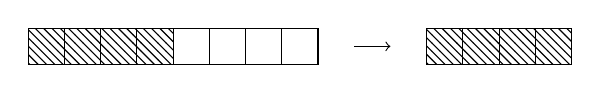
\begin{tikzpicture}[scale=.46]
        	\foreach \x in {0,...,7} {
        		\ifnum \x < 4
        			\filldraw[pattern=north west lines] (\x,0) rectangle (\x+1, 1);
        		\else
        			\draw (\x,0) rectangle (\x+1,1);
        		\fi
        	}
        	\draw[->] (9,0.5) -- (10,0.5);
        	\foreach \x in {0,...,3}
        			\filldraw[pattern=north west lines] (\x+11,0) rectangle (\x+12, 1);
        \end{tikzpicture}
        \end{center}
        
        If our program now adds an item to the dynamic array the same space needs to be
        allocated that was just freed, potentially moving all $2^{n-1}$ items. Imagine
        this delete-one/add-one cycle repeats, such as may happen with a stack backed
        by this dynamic array. Each append-one operation copies the (now) lower half to
        a new location, taking linear time on the number of items.
        
	\item The problem with that underflow strategy is that both the ``grow'' and
		``shrink'' events are at the same threshold---when half full, shrink by half thus
		making it full again, but this guarantees the next append will trigger a ``grow''.
		If the two thresholds are dissociated, we will avoid this pathological behavior.
		For this, only shrink the array to half size when it is a fourth full.
		
        \begin{center}
        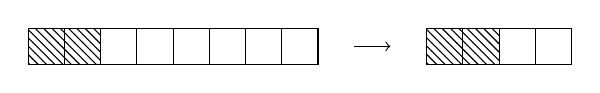
\begin{tikzpicture}[scale=.46]
        	\foreach \x in {0,...,7} {
        		\ifnum \x < 2
        			\filldraw[pattern=north west lines] (\x,0) rectangle (\x+1, 1);
        		\else
        			\draw (\x,0) rectangle (\x+1,1);
        		\fi
        	}
        	\draw[->] (9,0.5) -- (10,0.5);
        	\foreach \x in {0,...,3} {
        		\ifnum \x < 2
        			\filldraw[pattern=north west lines] (\x+11,0) rectangle (\x+12, 1);
        		\else
        			\draw (\x+11,0) rectangle (\x+12,1);
        		\fi
			}
        \end{tikzpicture}
        \end{center}
        
        We are then at the situation after a grow operation just duplicated the size of
        the array for us, thus amortizing the cost of grow/shrink operations.
\end{enumerate}

\paragraph{3-6}Skiena's fridge works as a stack, so unless he takes care of unstacking every food item regularly (thus emptying the fridge), that is bad news for the first items inserted.

One improvement might be to use a queue, whatever has been in there the longest is consumed first. However that is still a naive strategy---if an item expiring tomorrow is inserted after one that will expire in a year, I still risk the last item expiring.

The answer is a \emph{priority queue}. Prioritize the item that expires next. This ensures that items that have longer expiration dates wait the most.

\paragraph{3-7} The book says to keep a sentinel for the end of the list. There are three cases for delete: \begin{enumerate*}[label=\arabic*)]\item delete the first node; \item delete a node in the middle; \item delete the last node.\end{enumerate*}

\begin{enumerate}[label=\arabic*)]
	\item Deleting the head.
    \begin{center}
    \tikz[every rectangle node/.style={draw},
    	  every circle node/.style={draw}] {
    	\node[rectangle] (H) at (0,0) {H};
    	\node[circle] (1) at (1,0) {1};
    	\node[circle] (2) at (2,0) {2};
    	\node[rectangle] (T) at (3,0) {T};
    	\node[draw=white,scale=.7] (P) at (1,-0.7) {p};
    	\draw[->] (H) -- (1);
    	\draw[->] (1) -- (2);
    	\draw[->] (2) -- (T);
    	\draw[->] (P) -- (1);
    }
    \end{center}
    
    \lstinline!list.head == p!, point \lstinline!H! to \lstinline!p->next!, free \lstinline!p!
    
    \begin{center}
    \tikz[] {
    	\node[rectangle,draw] (H) at (0,0) {H};
    	\node[circle,draw=gray,dashed,gray] (1) at (1,0) {1};
    	\node[circle,draw] (2) at (2,0) {2};
    	\node[rectangle,draw] (T) at (3,0) {T};
    	\node[draw=white,scale=.7] (P) at (1,-0.7) {p};
    	\draw[->] (H) edge[bend left=45] (2);
    	\draw[->] (1) -- (2);
    	\draw[->] (2) -- (T);
    	\draw[->] (P) -- (1);
    }
    \end{center}

	\item Deleting a node in the middle of the list.
    \begin{center}
    \tikz[every rectangle node/.style={draw},
    	  every circle node/.style={draw}] {
    	\node[rectangle] (H) at (0,0) {H};
    	\node[circle] (0) at (1,0) {0};
    	\node[circle] (1) at (2,0) {1};
    	\node[circle] (2) at (3,0) {2};
    	\node[rectangle] (T) at (4,0) {T};
    	\node[draw=white,scale=.7] (P) at (2,-0.7) {p};
    	\draw[->] (H) -- (0);
	    \draw[->] (0) -- (1);
    	\draw[->] (1) -- (2);
    	\draw[->] (2) -- (T);
    	\draw[->] (P) -- (1);
    }
    \end{center}
    
    \lstinline;list.head != p;, \lstinline;p->next != tail;, overwrite \lstinline!p! with the content of \lstinline!p->next!, then free \lstinline!p->next!.

	\begin{center}    
    \tikz[] {
    	\node[rectangle,draw] (H) at (0,0) {H};
		\node[circle,draw] (0) at (1,0) {0};
    	\node[circle,draw] (1) at (2,0) {2};
    	\node[circle,draw=gray,dashed,gray] (2) at (3,0) {2};
    	\node[rectangle,draw] (T) at (4,0) {T};
    	\node[draw=white,scale=.7] (P) at (2,-0.7) {p};
    	\draw[->] (1) edge[bend left=45] (T);
		\draw[->] (H) -- (0);
		\draw[->] (0) -- (1);
    	\draw[->] (2) -- (T);
    	\draw[->] (P) -- (1);
    }
    \end{center}
    
    \item Deleting the last node.
    
    \begin{center}
    \tikz[every rectangle node/.style={draw},
    	  every circle node/.style={draw}] {
    	\node[rectangle] (H) at (0,0) {H};
    	\node[circle] (1) at (1,0) {1};
    	\node[circle] (2) at (2,0) {2};
    	\node[rectangle] (T) at (3,0) {T};
    	\node[draw=white,scale=.7] (P) at (2,-0.7) {p};
    	\draw[->] (H) -- (1);
    	\draw[->] (1) -- (2);
    	\draw[->] (2) -- (T);
    	\draw[->] (P) -- (2);
    }
    \end{center}
    
    \lstinline!p->next == tail!, free \lstinline!tail! and make \lstinline!p! the new sentinel node.
    
	\begin{center}    
    \tikz[] {
    	\node[rectangle,draw] (H) at (0,0) {H};
		\node[circle,draw] (1) at (1,0) {1};
    	\node[rectangle,draw] (2) at (2,0) {T};
    	\node[rectangle,draw=gray,dashed,gray] (T) at (3,0) {T};
    	\node[draw=white,scale=.7] (P) at (2,-0.7) {p};
		\draw[->] (H) -- (1);
    	\draw[->] (1) -- (2);
    	\draw[->] (P) -- (2);
    }
    \end{center}
\end{enumerate}

\paragraph{3-12} Maximum depth of a tree:
\begin{lstlisting}
data Tree = Node Tree Tree
          | Nil

maxDepth :: Tree -> Int
maxDepth Nil = 0
maxDepth (Node l r) = 1 + max (maxDepth l) (maxDepth r)
\end{lstlisting}

\paragraph{3-14} Merging two binary search trees into a doubly linked list. The in order
traversal of each tree provides ordered lists of their respective elements. A linear
sweep, choosing the minimum of each head and advancing in the chosen list will merge
the two structures. The cost of both the traversal and sweep/merge stages is $O(m+n)$,
where $m$ and $n$ are the number of elements in each binary search tree.

Note that this is fundamentally the idea behind mergesort.

\paragraph{3-15} There is presumably an insertion order that guarantees height balance.
Knowing all the elements and having them in order is a great advantage. Some thoughts:
clearly the extremes have to be inserted among the last few elements--their levels have
to be created for them to land in the right place. Also, the median element of the array
has to be the root, as it gives the most ``space'' to its sides.

That median element determines two halves. Each half has its own median element to which
the same thinking process applies. Therefore a potential algorithm for building a height balanced tree is:
\begin{lstlisting}
balanced_insertion(lo, hi):
  m <- median(lo, hi)
  insert element m
  balanced_insertion(lo, m-1)
  balanced_insertion(m+1, hi)
\end{lstlisting}
With some provisions for ranges of length 1, in which case the element is a leaf and can
be inserted with no further recursive calls.

Before doing the insertion, the binary search tree has to be traversed in order to build
an array of all its elements. This takes $O(n)$ time.

Consider the call stack of \lstinline!balanced_insertion()! with the full range of $n$
elements. It makes two recursive calls, so the call stack is shaped like
a binary tree. The height of the call tree is at most $\lg n$, because the range of
elements in each recursive call is more than halved with respect to the range of its
caller. Then this tree can have at most $2^{1+\lg n} = 2\cdot 2^{\lg n} = 2n$ nodes, each
representing a call to \lstinline!balanced_insertion()!. Since each call does constant time work, this function's running time is $O(n)$ as well.

\paragraph{3-17} The definition of height balanced tree is recursive, but the recursive
aspect is implicit in the way it's worded in the book. An explicit way to say it is: a
binary tree is height balanced if both its children are height balanced and the difference
between their heights is at most 1. A node with no children is balanced and has height 1
(or, equivalently, a ``null'' node is balanced and has height 0).

\begin{lstlisting}
data Tree = Node Tree Tree
          | Nil

isBalanced :: Tree -> (Bool, Int)
isBalanced Nil = (True, 0)
isBalanced (Node l r) = (balanced, height)
  where (lb, lh) = isBalanced l
        (rb, rh) = isBalanced r
        height   = 1 + max lh rh
        balanced = lb && rb && abs (lh - rh) <= 1
\end{lstlisting}

Each call performs constant-time work, and there is only one call for each node in the
tree. Therefore this is an $O(n)$ time algorithm.

\paragraph{3-18} We have a balanced tree where all of \lstinline!search()!,
\lstinline!insert()!, \lstinline!delete()!, \lstinline!minimum()! and
\lstinline!maximum()! take $O(\log n)$ time, and we want to ensure it supports
\lstinline!successor()! and \lstinline!predecessor()! in $O(1)$ time. Each node will
have pointers to its logical predecessor and successor that will have to be
maintained during update operations. This would effectively add a doubly linked list
structure on top of the binary tree.

%\begin{forest}
%	[5
%		[3 [2 [1]] [4]]
%		[7 [6] [8]]]
%\end{forest}

\lstinline!successor()!: see pp. 85 in the book. The in order successor can be found, with
a parent pointer, by considering two different cases: if the node has a right subtree, and
if it hasn't.

\lstinline!predecessor()!: finding it is symmetric to the successor.
\begin{itemize}
	\item If a node is a leaf, and is the left child of its parent, traverse up until 
		finding a node that is the right child of its parent. The parent will be the 
		predecessor.
	\item If a node is a leaf and is a right child, this is the trivial case of the
		previous point---the parent is the predecessor.
	\item If a node has a left subtree, the predecessor is the maximum of that left
		subtree.
\end{itemize}

When deleting an item from the tree, we can get ahold of its successor and predecessor
in $O(1)$ time via the pointers, delete the item, then link the pointers as done in a
doubly linked list.

Note that the exercise says the tree is balanced. We can assume there is a balancing
operation that takes place after each insert and delete, before the successor and
predecessor pointers are updated.

\paragraph{3-19} We have a dictionary with $O(\log n)$ \lstinline!search()!,
\lstinline!insert()!, \lstinline!delete()!, \lstinline!min()!, \lstinline!max()!,
\lstinline!predecessor()! and \lstinline!successor()!, and we want to make some changes
to \lstinline!insert()! and \lstinline!delete()! so \lstinline!min()! and \lstinline!max()!
will take $O(1)$ time while the update operations still take $O(\log n)$ time.

After \lstinline!insert()! we can query for the new element's predecessor in $O(\log n)$
time---if there isn't one, our new element is the new minimum. Similarly with
\lstinline!maximum()! and \lstinline!successor()!.

Before \lstinline!delete()! we can query for the predecessor of the element---if there
isn't one we can find the new minimum by querying for its successor (although in reality
we'd know we are trying to delete the minimum because we have a $O(1)$ minimum); likewise
when deleting the maximum. If before delete we do find a more extreme element, we know
we are not deleting the minimum or maximum and no adjustment is necessary.

\paragraph{3-20} The exercise calls this structure a ``set'', and by its operations it
does look like a set, so we'll assume the elements are unique. Furthermore, we will assume
we have a balancing operation that keeps the tree height balanced in $O(\log n)$ time.

Our set structure is backed by a balanced binary search tree. The \lstinline!member()!
query searches for the element, taking $O(\log n)$ time. The \lstinline!insert()!
operation is the regular BST insert---if the key already exists, it is overwritten; this
also takes $O(\log n)$ time. Finally, \lstinline!delete()! has to find the $k$-th smallest
element. Assume our BST has $O(\log n)$ \lstinline!minimum()! and $O(1)$ \lstinline!successor()!,
as in the previous exercise. Then we need to query for the minimum element and then $k$
calls to \lstinline!successor()!, then one $O(\log n)$ delete and one $O(\log n)$
rebalance.

Unfortunately this doesn't work---consider always deleting the last element. After finding
the minimum, we always do $n$ calls to \lstinline!successor()!, turning this into a $O(n)$
algorithm in the worst case. \lstinline!:\!

\paragraph{3-21} This may be cheating somehow, but if the two sets are disjoint and all
keys in $S_1$ are less than every key in $S_2$, we can concatenate both trees by finding
the minimum element in $S_2$ and making the root of $S_1$ its left child. It would wreak
havoc on the balance of the tree, but rebalancing should take at most $O(n+m)$ time, for
$n$ elements in $S_1$ and $m$ elements in $S_2$. The traversal of $S_2$ to its
minimum would be $O(log m)$ and the concatenation---a simple matter of pointer
manipulation---would be constant time.

\paragraph{3-22} We have to design a data structure that supports \lstinline!insert(x)!
and \lstinline!median()! operations, both in $O(\log n)$ time. Inserting is easy enough,
but the median is an element relative to all other elements in the structure; it depends
on its logical position within the set of all the elements, so it's not clear that it
can be determined without somehow keeping track of counts.

Suppose the structure keeps two binary search trees, the median, and counters for the
elements in each tree. The elements in the left tree are less than the median, while
those on the right tree are greater than the median.

When inserting, we compare the element to the median to select which side to insert it
into. It's then inserted in the correct tree, taking $O(\log n)$ time (actually $\log m$,
with $m$ the number of elements on that side of the median). We increase the counter on
this side, and if the difference in elements between both sides is greater than 1, we
know we need to shift the median.

To rebalance the structure, suppose the left side has two more elements than the right
side. We can insert the median in the right tree in $O(\log n)$ time, then find and
delete the maximum from the left tree, also in $O(\log n)$ time, and set it as the new
median. The right counter increases by one, the left counter decreases by one, and we are
balanced again.

This actually gives $O(1)$ access to the median, so it is probably wrong for the exercise.

\chapter{Sorting}

\section{Solutions}

\paragraph{4-1} The Grinch wants the most unbalanced game possible. This is the same as asking to maximize the difference in total skill between the two teams.

In $O(n\log n)$, sort the player pool by skill and make each half of the result a team. Any swap between teams would bring a higher skilled player into the lower half, and a lower skilled player into the higher half, making the difference in total skill lower.

\paragraph{4-2}
\begin{enumerate}[label=(\alph*)]
	\item Unsorted array. Find $x, y$ that maximize $|x-y|$ in $O(n)$ time. In one sweep through the array, find the minimum and maximum values. These maximize the difference.
	\item Sorted array. Find $x, y$ that maximize $|x-y|$ in $O(1)$ time. These are the first and last elements of the array.
	\item Unsorted array. Find $x, y$ that minimize $|x-y|$, for $x\ne y$, in $O(n\log n)$ time. Sort the array in $O(n\log n)$ then do a linear pairwise search of consecutive values for the pair with the smallest difference in $O(n)$ time.
	\item Sorted array. Find $x, y$ that minimize $|x-y|$, for $x\ne y$, in $O(n)$ time. Do a pairwise comparison of every element with the next in $O(n)$ and find the consecutive pair with the smallest difference.
\end{enumerate}

\paragraph{4-3} What we want to do here is first sort the array in $O(n\log n)$ time. Then we want to pair up the biggest offender with the least problematic number, so the largest with the smallest, the second largest with the second smallest, and so on.
\begin{equation*}
	x_1 < x_2 < \ldots < x_{2n-1} < x_{2n} \quad\rightarrow\quad (x_1, x_{2n}), (x_2, x_{2n-1}), \ldots
\end{equation*}

Why does this work? Suppose in my pairing I find that $(x,y)$ are my maximum pair. By way of contradiction, I claim that there is a different partition of the $2n$ numbers whose maximum pair is less than $(x,y)$.

Let's say that $x<y$. The claim that a different partition does better implies that, whatever its maximum pair is, element $y$ in this hypothetical partition has to be paired up with an element $t$ such that $t<x$, otherwise the maximum pair could not be less than $x+y$. But the same logic applies to every element larger than $y$. They need to be paired up with elements smaller than $x$ certainly, or for any $z>y$ we'd have a pair $(z,x)$ where $z+x > x+y$ is larger than the claimed maximum.

Now suppose there are $i$ elements larger than $y$. In my original pairing, that means there are $i$ elements smaller than $x$. But the claim forced me to pair $y$ with one of those $i$ elements smaller than $x$, so there are now $i-1$ numbers available to pair with the $i$ numbers larger than $y$. We see that we won't be able to find pairs for every element that don't surpass our claimed maximum pair. The contradiction shows that our original pairing was indeed optimal, and the algorithm correct.

















\end{document}